%%%%%%%%%%%%%%%%%%%%%%%%%%%%%%%%%%%%%%%%%
% University Assignment Title Page 
% LaTeX Template
% Version 1.0 (27/12/12)
%
% This template has been downloaded from:
% http://www.LaTeXTemplates.com
%
% Original author:
% WikiBooks (http://en.wikibooks.org/wiki/LaTeX/Title_Creation)
%
% License:
% CC BY-NC-SA 3.0 (http://creativecommons.org/licenses/by-nc-sa/3.0/)
% 
% Instructions for using this template:
% This title page is capable of being compiled as is. This is not useful for 
% including it in another document. To do this, you have two options: 
%
% 1) Copy/paste everything between \begin{document} and \end{document} 
% starting at \begin{titlepage} and paste this into another LaTeX file where you 
% want your title page.
% OR
% 2) Remove everything outside the \begin{titlepage} and \end{titlepage} and 
% move this file to the same directory as the LaTeX file you wish to add it to. 
% Then add \input{./title_page_1.tex} to your LaTeX file where you want your
% title page.
%
%%%%%%%%%%%%%%%%%%%%%%%%%%%%%%%%%%%%%%%%%
%\title{Title page with logo}
%----------------------------------------------------------------------------------------
%	PACKAGES AND OTHER DOCUMENT CONFIGURATIONS
%----------------------------------------------------------------------------------------

\documentclass[12pt]{article}
\usepackage[english]{babel}
\usepackage[utf8x]{inputenc}
\usepackage{amsmath}
\usepackage{graphicx}
\usepackage[colorinlistoftodos]{todonotes}

\begin{document}

\begin{titlepage}

\newcommand{\HRule}{\rule{\linewidth}{0.5mm}} % Defines a new command for the horizontal lines, change thickness here

\center % Center everything on the page
 
%----------------------------------------------------------------------------------------
%	HEADING SECTIONS
%----------------------------------------------------------------------------------------

\textsc{\LARGE Politenico di Milano}\\[1.5cm] % Name of your university/college
\textsc{\Large Dipartimento Elettronica, Informazione e Bioingegneria}\\[0.5cm] % Major heading such as course name
\textsc{\large HEAPLab Project Report}\\[0.5cm] % Minor heading such as course title

%----------------------------------------------------------------------------------------
%	TITLE SECTION
%----------------------------------------------------------------------------------------

\HRule \\[0.4cm]
{ \huge \bfseries EdgeCloudSim Report}\\[0.4cm] % Title of your document
\HRule \\[1.5cm]
 
%----------------------------------------------------------------------------------------
%	AUTHOR SECTION
%----------------------------------------------------------------------------------------

\begin{minipage}{0.4\textwidth}
\begin{flushleft} \large
\emph{Author:}\\
Zhang \textsc{Qiaolun} % Your name
\end{flushleft}
\end{minipage}
~
\begin{minipage}{0.4\textwidth}
\begin{flushright} \large
\emph{Supervisor:} \\
Michele \textsc{Zanella} % Supervisor's Name
\end{flushright}
\end{minipage}\\[2cm]

% If you don't want a supervisor, uncomment the two lines below and remove the section above
%\Large \emph{Author:}\\
%John \textsc{Smith}\\[3cm] % Your name

%----------------------------------------------------------------------------------------
%	DATE SECTION
%----------------------------------------------------------------------------------------

{\large \today}\\[2cm] % Date, change the \today to a set date if you want to be precise

%----------------------------------------------------------------------------------------
%	LOGO SECTION
%----------------------------------------------------------------------------------------


\includegraphics[width=100pt]{heaplogo.pdf}\\[1cm] % Include a department/university logo - this will require the graphicx package
 
%----------------------------------------------------------------------------------------

\vfill % Fill the rest of the page with whitespace

\end{titlepage}




\begin{abstract}
The simulation tool EdgeCloudSim provides some basic features of simulating edge computing scenarios. But it lacks some further features. This project extends basic task application definition to support task-based application.
\end{abstract}

\section{Introduction}

EdgeCloudSim is a simulation tool which can simulate Edge Computing scenarios. But this tool can not simulate task-based application. The project adds the following features to the simulation tool:

\begin{enumerate}
	\item Extend basic task application definition to support task-based application
	\item Task migration among the Edge or Cloud VMs
	\item Add probabilistic network failure model by considering the congestion or other parameters such as the distance between mobile device and the WiFi access point.
	\item Visual tool for displaying the network topology
\end{enumerate}


In the end, this project gives a detailed simulation and provides the simulation results.


\section{Relation between EdgeCloudSim and Cloudsim}

\subsection{Simulation Framework of CloudSim}
\subsubsection{Simulation Data Flow}
CloudSim is a discrete event management framework. The core simulation process is a loop function which checks the events related to all the entities and processes the event. Each entities can process different kinds of events. So figuring out all the 

\subsubsection{Data center internal processing}
\begin{figure}
	\centering
	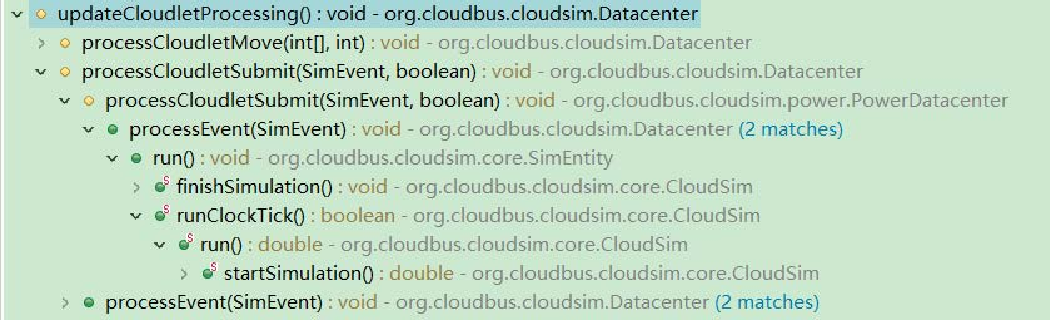
\includegraphics[width=1\textwidth]{./figures/2-updateCloudletProcessing.pdf}
	\caption{\label{fig:cloudletProcessing}Call hierarchy of function updateCloudletProcessing.}
\end{figure}

Figure 1 shows the call hierarchy of member function updateCloudletProcessing in class DataCenter. From this figure, we can figure out that the Cloudlet processing update process figure in the paper about CloudSim is wrong. Figure 2 is the fixed Cloudlet processing update process. At the end of the function updateCloudletProcessing, it will add a new VM\_DATACENTER\_EVENT to the future queue using function schedule. When we go back to the loop of Run function, the updateCloudletProcessing function will be triggered again.

\begin{figure}
	\centering
	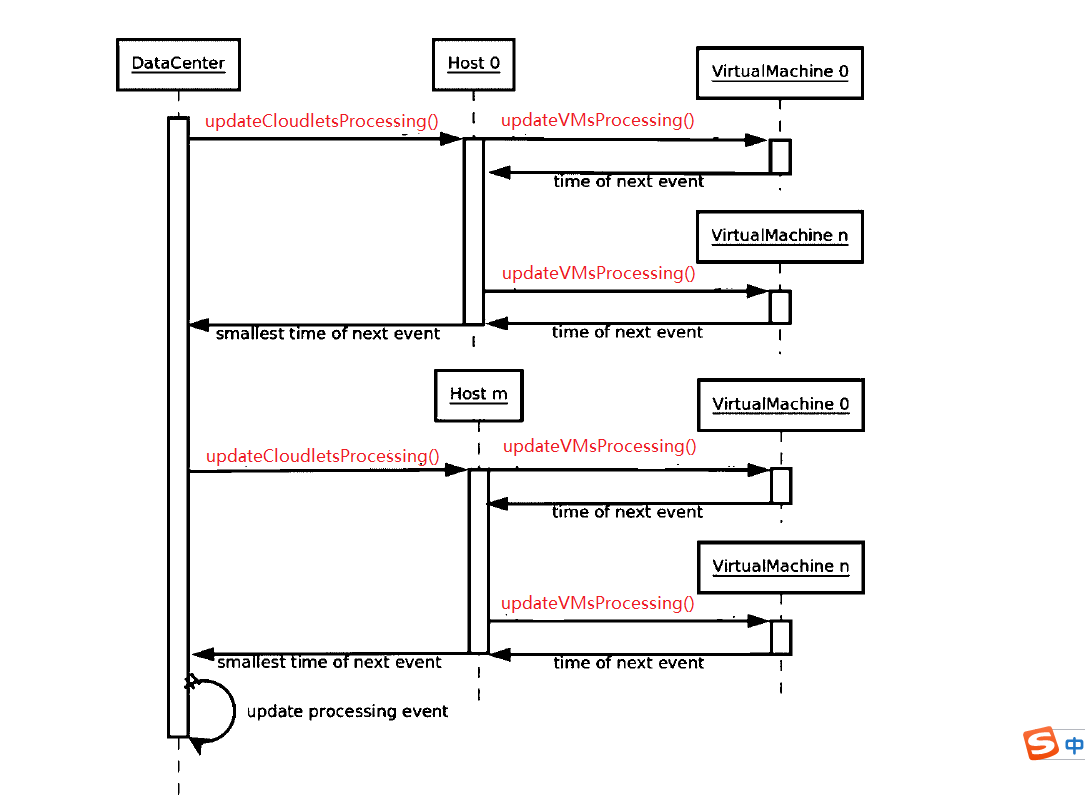
\includegraphics[width=1\textwidth]{./figures/3-processingSequence.png}
	\caption{\label{fig:processingSequence}Cloudlet processing update process.}
\end{figure}

\subsection{Simulation Framework of EdgeCloudSim}
\begin{figure}
	\centering
	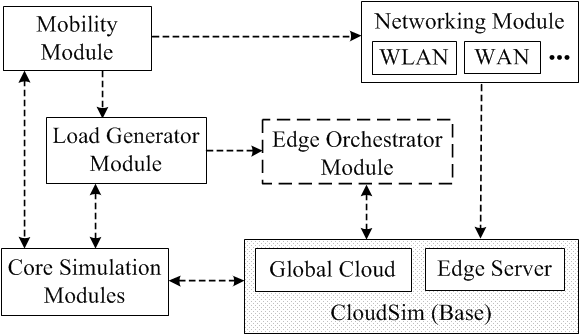
\includegraphics[width=1\textwidth]{./figures/1-edgecloudsim_diagram.png}
	\caption{\label{fig:frog}This is a figure caption.}
\end{figure}

As is shown in the picture1, there are two important classes in core package: ScenarioFactory and SimManager. The ScenarioFactory gets the parameters for the scenarios. And the SimManager receives the object of type ScenarioFactory. Moreover, the SimManager is a class extended from SimEntity class. The SimEntity is a class defined in CloudSim. And it has a function called startEntity(), which will schedule the task. 
\todo[inline, color=green!40]{Not sure if I can implement the task-based application here or change the schedule function in CloudSim}

\subsection{Modules in EdgeCloudsim}
\begin{enumerate}
	\item core: three are there important class in this module. ScenarioFactory.java is the class for factory scheme. SimManager.java class extends SimEntity class and it is related to CREATE\_TASK, CHECK\_ALL\_VM, GET\_LOAD\_LOG, PRINT\_PROGRESS, STOP\_SIMULATION. SimSettings.java is the class that stores all the configurations.
	\item cloud\_server: class CloudServerManager.java. This class actually just generate the hostlist, vmlist, local data center, and function to get the average utilization of all VMS. 
	\item edge\_server: class EdgeServerManager.java has similar functions as CloudServer.
	\item mobile\_processing: class MobileServerManager.java. This class enables the mobile devices have the ability to process task. We can also create data centers and virtual machines on it.
	\item edge\_client: MobileDeviceManager.java extends DatacenterBroker class in CloudSim. And it overwrite the processOtherEvent function and add new events: REQUEST\_RECEIVED\_BY\_CLOUD, REQUEST\_RECEIVED\_BY\_EDGE\_EDGE\_DEVICES.
\end{enumerate}


\subsection{Entities in EdgeCloudsim}
\begin{enumerate}
	\item SimManager: public class SimManager extends SimEntity
	\item MobileDeviceManager: public abstract class MobileDeviceManager  extends DatacenterBroker
	\item EdgeOrchestrator: public abstract class EdgeOrchestrator extends SimEntity
\end{enumerate}


\subsection{Relationship of Modules between CloudSim and EdgeCloudSim}
Because EdgeCloudSim is implemented on the top of CloudSim, it also relies on the discrete event management framework. 
MobileDeviceManager class extends DatacenterBroker class. So it implemented the following functions


\section{Design and Implementation}

\subsection{Task-based Application Design and Implementation}

\subsubsection{Task-based Application Design}
In EdgeCloudSim, task is atomic and cannot be divided into smaller tasks. Task-based application is an application which is composed by several smaller This project designs how to introduce a task-based 
What is task-based application
Introduce task-dependency graph

\subsubsection{Scheduling Algorithm in EdgeCloudSim}
Which module can we modify to achieve task-based application?
How to deal with task-dependency graph

\subsubsection{Component Diagram of the Simulation tool}
After adding the feature, the component diagram has changed.

\subsection{Task Migration}

\subsection{Probabilistic Network Failure Model}

\section{Experimental Results}
In this section, we did some experiment. We test the failure rate.

\section{Conclusions}


\section{Some \LaTeX{} Examples}
\label{sec:examples}

\subsection{Sections}

Use section and subsection commands to organize your document. \LaTeX{} handles all the formatting and numbering automatically. Use ref and label commands for cross-references.

\subsection{Comments}

Comments can be added to the margins of the document using the \todo{Here's a comment in the margin!} todo command, as shown in the example on the right. You can also add inline comments too:

\todo[inline, color=green!40]{This is an inline comment.}

\subsection{Tables and Figures}

Use the table and tabular commands for basic tables --- see Table~\ref{tab:widgets}, for example. You can upload a figure (JPEG, PNG or PDF) using the files menu. To include it in your document, use the includegraphics command as in the code for Figure~\ref{fig:frog} below.

% Commands to include a figure:
\begin{figure}
\centering
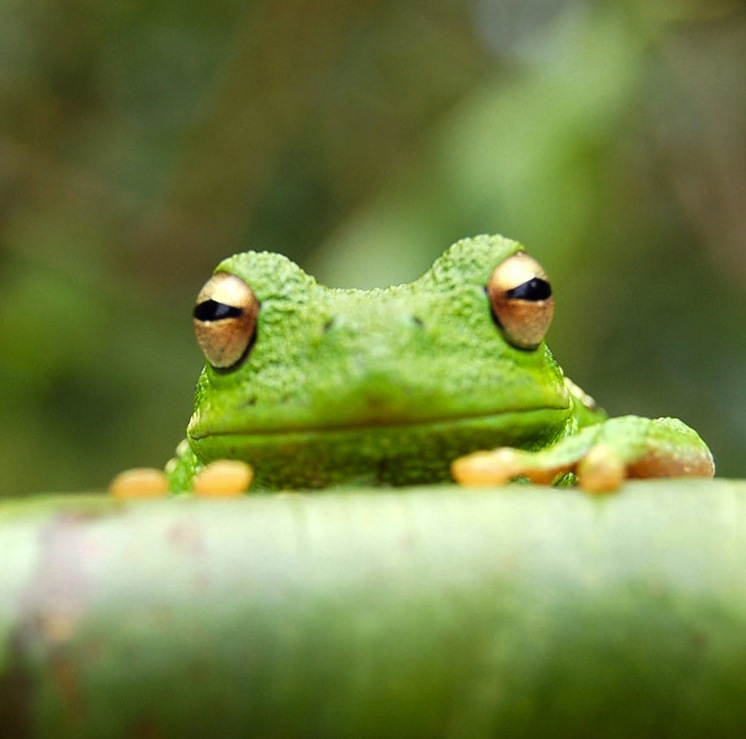
\includegraphics[width=0.5\textwidth]{frog.jpg}
\caption{\label{fig:frog}This is a figure caption.}
\end{figure}

\begin{table}
\centering
\begin{tabular}{l|r}
Item & Quantity \\\hline
Widgets & 42 \\
Gadgets & 13
\end{tabular}
\caption{\label{tab:widgets}An example table.}
\end{table}

\subsection{Mathematics}

\LaTeX{} is great at typesetting mathematics. Let $X_1, X_2, \ldots, X_n$ be a sequence of independent and identically distributed random variables with $\text{E}[X_i] = \mu$ and $\text{Var}[X_i] = \sigma^2 < \infty$, and let
$$S_n = \frac{X_1 + X_2 + \cdots + X_n}{n}
      = \frac{1}{n}\sum_{i}^{n} X_i$$
denote their mean. Then as $n$ approaches infinity, the random variables $\sqrt{n}(S_n - \mu)$ converge in distribution to a normal $\mathcal{N}(0, \sigma^2)$.

\subsection{Lists}

You can make lists with automatic numbering \dots

\begin{enumerate}
\item Like this,
\item and like this.
\end{enumerate}
\dots or bullet points \dots
\begin{itemize}
\item Like this,
\item and like this.
\end{itemize}

We hope you find write\LaTeX\ useful, and please let us know if you have any feedback using the help menu above.

\end{document}